\chapter{Drools Concept hierarchy}
\label{appendix:DroolsConceptHierarchy}

The concept hierarchy presented on the following pages was extracted and interpreted from Drools railroad diagrams.

The diagram in figure \ref{fig:RuleFileDiagram} represents the file level and can be considered the root of concept hierarchy.
This hierarchy represents the concepts that are available to the rule file.
As the only concept that we will examine in depth is the rule, we show some shared concepts or children of, for example, function, query and type declaration.

In our final implementation, the only children of File we implemented were the Import, Global and Rule concepts.

The diagram in figure \ref{fig:RuleDiagram} shows the children of a rule.
Each attribute has a different Behavior and Structure and are thus all represented separately.

In these diagrams, we do not show a concept diagram for the RHS.
This choice was because it would be more or less the concept diagram for Java Statements, with the addition of Rule Variables and some special Drools functions.
The concept diagram for a General Purpose Language would be orders of magnitude more extensive and more complex than we wish to show here.
Luckily, as MPS allows for almost seamless extension and integration of different languages, we can import JetBrains implementation of Java for the RHS.

We show the hierarch for the LHS in the diagram in figure \ref{fig:LHSDiagram}.
Because of the number of concepts being represented, it may be a little hard to read.

 

\begin{figure}
    \centering
    \fbox{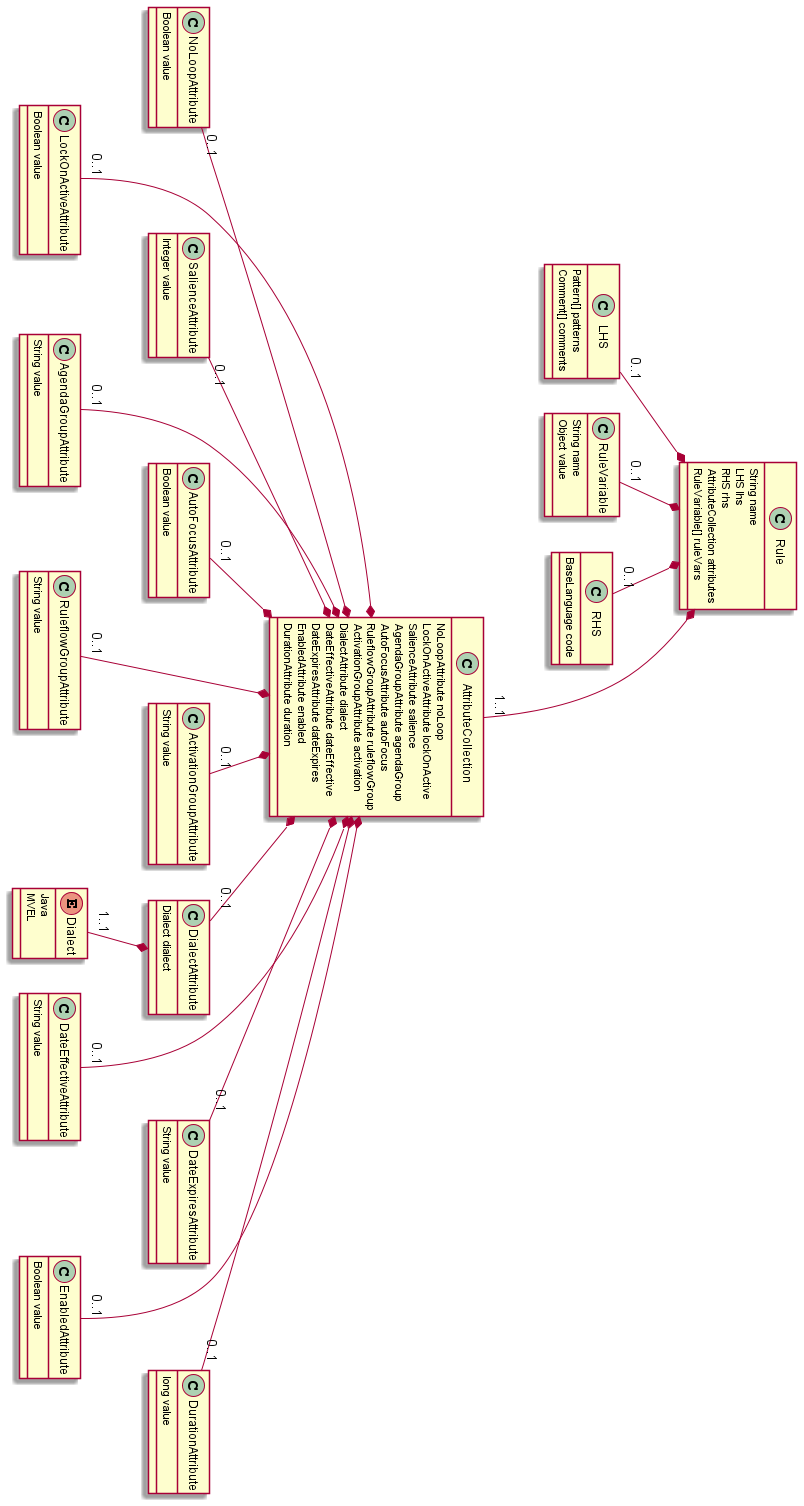
\includegraphics[width=0.80\textwidth]{Appendices/images/Droolsstructurerules.png}}
    \caption{Rules concept hierarchy diagram}
    \label{fig:RuleDiagram}
\end{figure}
 

\begin{figure}
    \centering
    \fbox{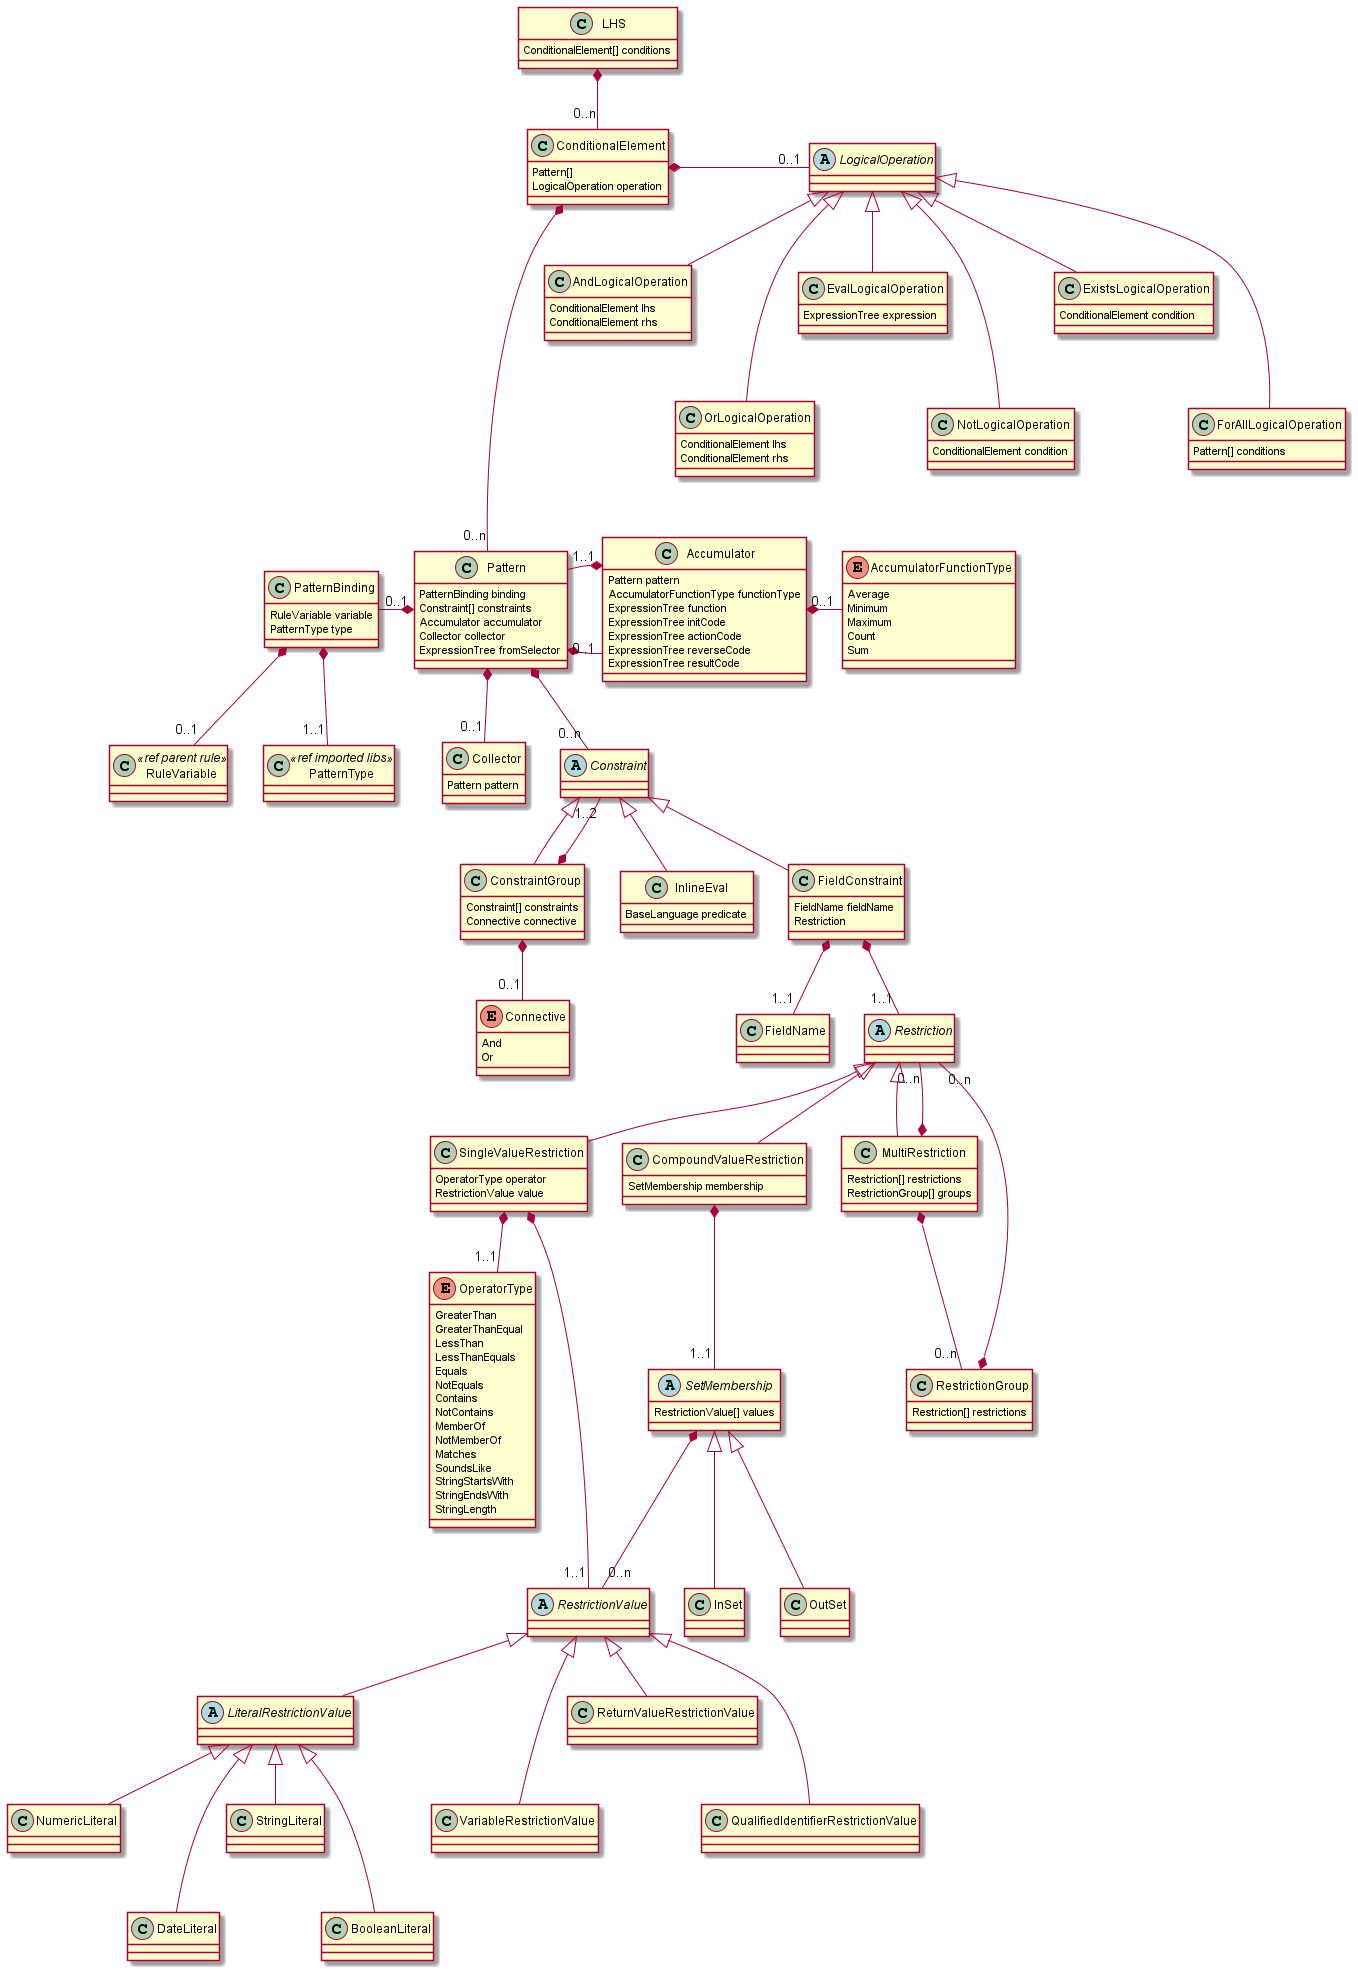
\includegraphics[width=0.99\textwidth]{Appendices/images/DroolsStructureLHS.png}}
    \caption{Rule LHS concept hierarchy diagram}
    \label{fig:LHSDiagram}
\end{figure}
 